\documentclass[UTF8,a4paper,12pt]{ctexart}

\usepackage{amsmath,amssymb}
\usepackage{geometry}
\usepackage{xcolor}
\usepackage{listings}
\usepackage{booktabs}
\usepackage{graphicx}
\usepackage{hyperref}

\geometry{left=2.8cm,right=2.8cm,top=2.6cm,bottom=2.6cm}
\graphicspath{{figures/}}
\emergencystretch=2em
\newcommand{\thinktag}{\texttt{<think>\allowbreak...\allowbreak</think>}}

\lstset{
  basicstyle=\ttfamily\small,
  keywordstyle=\color{blue!70!black},
  commentstyle=\color{green!40!black},
  stringstyle=\color{orange!80!black},
  numbers=left,
  numberstyle=\tiny\color{gray},
  frame=single,
  breaklines=true,
  columns=fullflexible,
  keepspaces=true
}

\title{2.9 面向机器学习任务的数据准备流程与 Python 实操}
\author{Chapter 2.9}
\date{\today}

\begin{document}

\begin{center}
  {\LARGE \textbf{2.9 面向机器学习任务的数据准备流程与 Python 实操}}\\[0.4em]
  {\large 从原始对话记录到可训练 JSONL 样本}
\end{center}

\section*{第一页：数据清洗要先回答“样本是什么”}

本节的实操任务是把一组脱敏对话记录整理成大模型监督微调样本。这里的关键不是字段越多越好，而是先明确样本单位：一条可训练样本应当包含一个用户输入和一个清洗后的模型回答。因此，原始数据需要被转换为：
\[
  \text{原始记录} \longrightarrow (\texttt{id},\ \texttt{instruction},\ \texttt{input},\ \texttt{output},\ \texttt{metadata})
\]

围绕这个目标，清洗流程可以压缩成四步：读入数据并理解字段结构；从对话字段中抽取有效问答对；处理噪声，包括推理草稿、异常长度和重复样本；记录每一步之后还剩多少样本。实操中最值得强调的是：\thinktag{} 这类内容不应机械地保留在最终回答里，长度过滤也不是随手删数据，而是在控制训练信号的质量。

\begin{figure}[htbp]
  \centering
  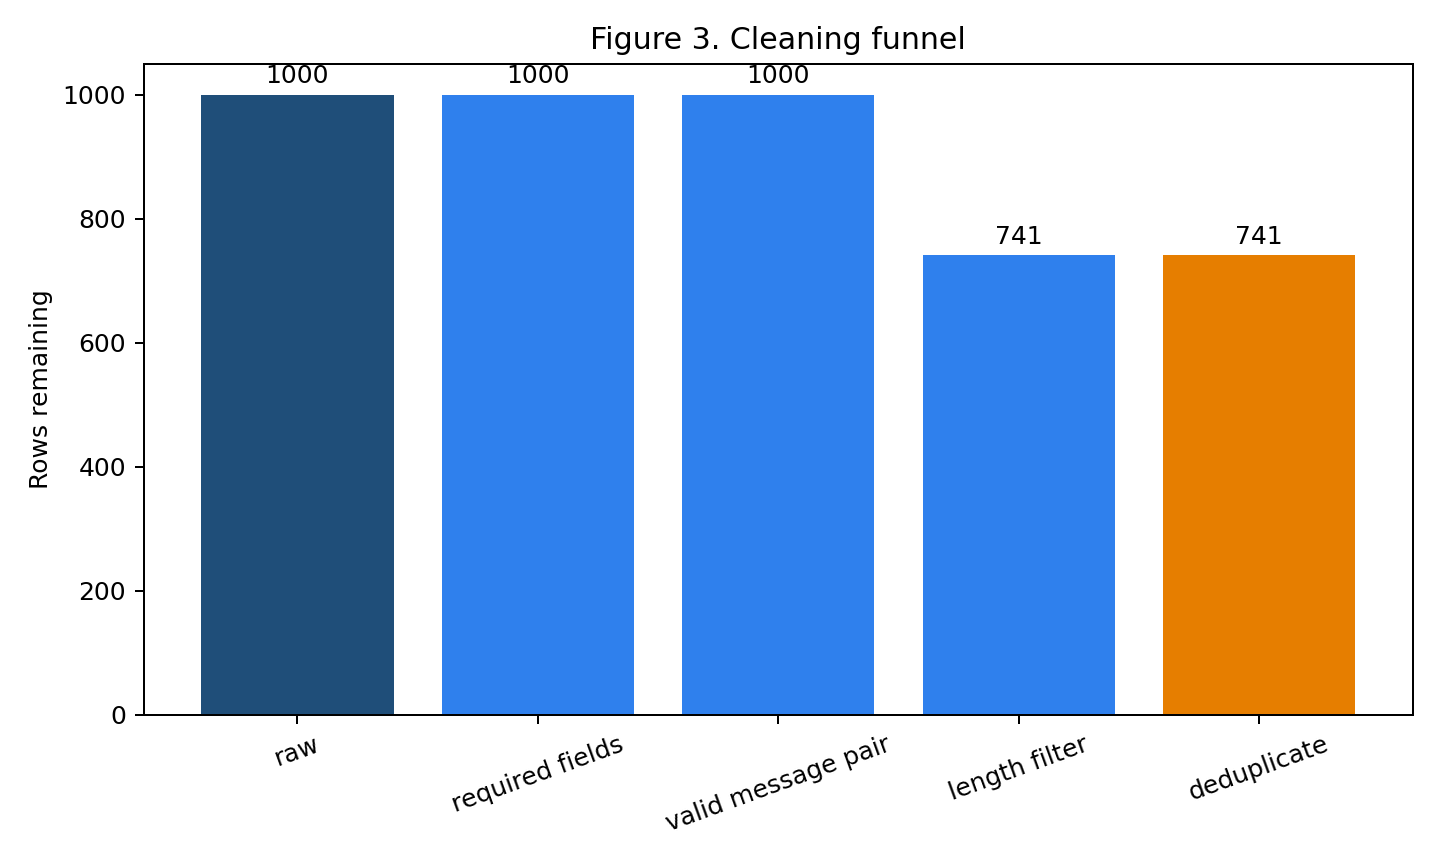
\includegraphics[width=0.72\linewidth]{fig3_cleaning_funnel.png}
  \caption{从原始数据到可训练样本的清洗漏斗}
\end{figure}

图 1 展示了清洗漏斗：1000 条原始样本依次经过关键字段检查、有效问答抽取、长度过滤和去重，最终保留 741 条。它要传达的重点不是某个阈值本身，而是清洗过程必须可追踪：每一步删掉了什么、为什么删、删完之后数据规模如何变化，都应该能被解释。

\newpage

\section*{第二页：清洗后的数据还要能支撑实验}

清洗完成并不意味着数据准备结束。机器学习实验还需要明确训练、验证和测试边界，否则后续评价很容易混乱。本节将 741 条清洗样本按 80\%、10\%、10\% 划分，并固定随机种子，使后续实验能够复现。

\begin{figure}[htbp]
  \centering
  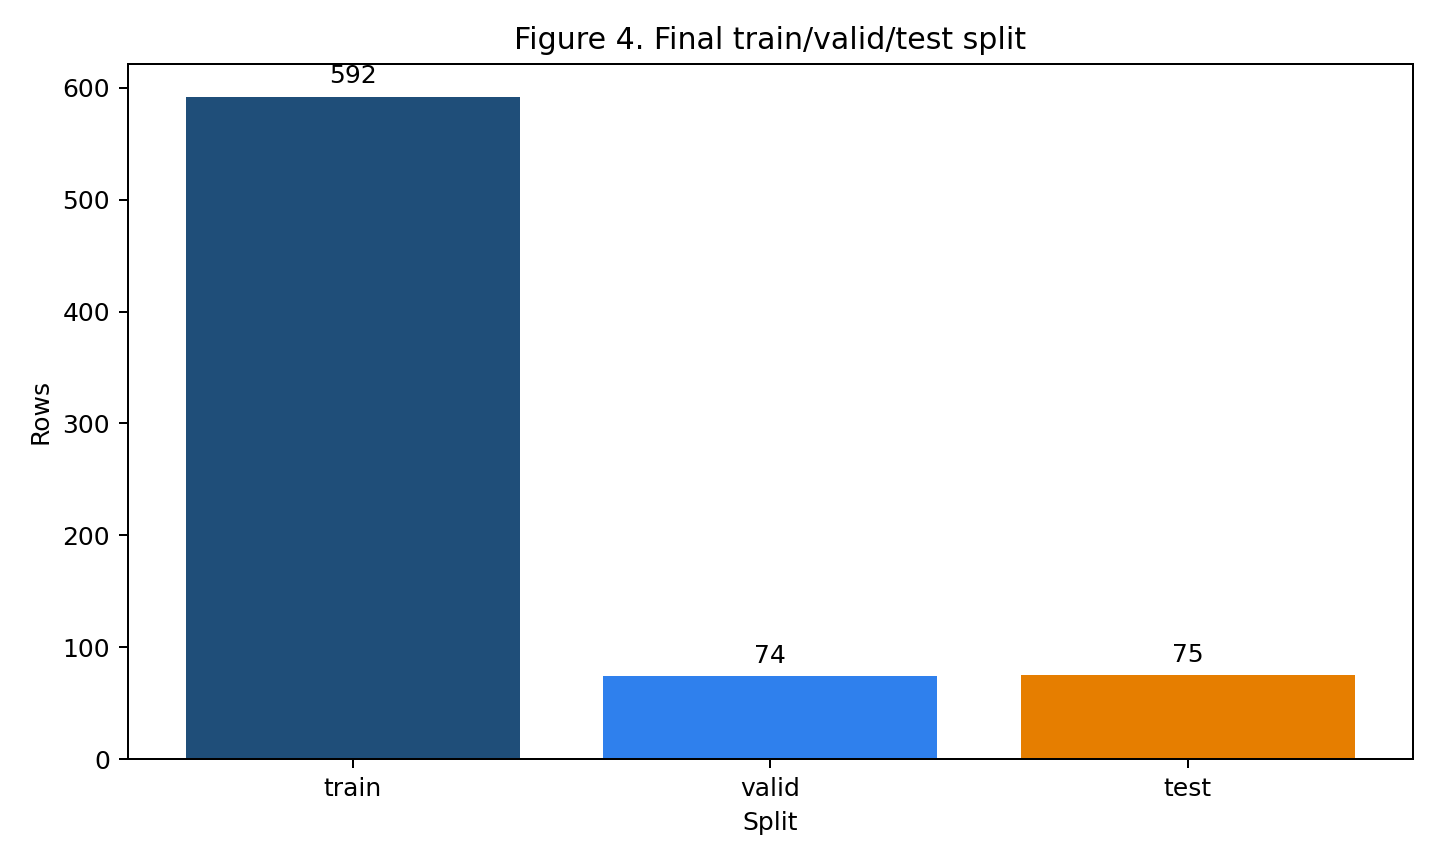
\includegraphics[width=0.70\linewidth]{fig4_final_split.png}
  \caption{清洗后样本的训练、验证、测试划分}
\end{figure}

图 2 给出了最终划分结果：训练集 592 条，验证集 74 条，测试集 75 条。这里的重点不是比例本身，而是清洗规则和划分规则必须固定。若先观察测试集效果，再反复调整长度阈值、去重规则或推理块处理方式，测试集就会被间接用于调参，评价结果也会变得不可靠。

这节课真正需要带走的是一条通用主线：

\begin{enumerate}
  \item \textbf{先定义任务：}模型要学什么，样本单位就是什么。
  \item \textbf{再理解数据：}字段名只是入口，真正重要的是字段如何构成输入、输出和标签。
  \item \textbf{然后清洗质量问题：}缺失、噪声、异常、重复都会改变训练信号。
  \item \textbf{最后固定实验边界：}记录规则、数量变化、划分比例和随机种子。
\end{enumerate}

因此，数据清洗不是建模前的附属工作，而是实验设计的一部分。只有样本单位清楚、清洗规则清楚、数量变化清楚，数据才真正具备进入训练和评价的条件。

\end{document}
